\documentclass{article}

\usepackage{fancyhdr} % Required for custom headers
\usepackage{lastpage} % Required to determine the last page for the footer
\usepackage{extramarks} % Required for headers and footers
\usepackage[usenames,dvipsnames]{color} % Required for custom colors
\usepackage{graphicx} % Required to insert images
\usepackage{listings} % Required for insertion of code
\usepackage{courier} % Required for the courier font
\usepackage{lipsum} % Used for inserting dummy 'Lorem ipsum' text into the template
\usepackage{amsmath}
\usepackage{amssymb}
\usepackage{mathtools, xparse}
\usepackage{booktabs}
\usepackage{bigstrut}
\usepackage{float}
\usepackage{hyperref}
\usepackage{color}
\usepackage{algorithm}
\usepackage{caption}
\usepackage{algpseudocode}
\usepackage{multirow}


\DeclarePairedDelimiter{\norm}{\lVert}{\rVert}
\DeclarePairedDelimiter\abs{\lvert}{\rvert}%

\hypersetup{
    colorlinks   = true,    % Colours links instead of ugly boxes
    urlcolor     = red,    % Colour for external hyperlinks
    linkcolor    = red,    % Colour of internal links
    citecolor    = red      % Colour of citations
}
% Margins
\topmargin=-0.45in
\evensidemargin=0in
\oddsidemargin=0in
\textwidth=6.5in
\textheight=9.0in
\headsep=0.25in

\linespread{1.1} % Line spacing

% Set up the header and footer
\pagestyle{fancy}
\lhead{\hmwkAuthorName} % Top left header
\chead{\hmwkClass\ : \hmwkID} % Top center head
\rhead{\firstxmark} % Top right header
\lfoot{\lastxmark} % Bottom left footer
\cfoot{} % Bottom center footer
\rfoot{Page\ \thepage\ of\ \protect\pageref*{LastPage}} % Bottom right footer
\renewcommand\headrulewidth{0.4pt} % Size of the header rule
\renewcommand\footrulewidth{0.4pt} % Size of the footer rule

\setlength\parindent{0pt} % Removes all indentation from paragraphs

%----------------------------------------------------------------------------------------
%	CODE INCLUSION CONFIGURATION
%----------------------------------------------------------------------------------------

\definecolor{MyDarkGreen}{rgb}{0.0,0.4,0.0} % This is the color used for comments
\lstloadlanguages{Perl} % Load Perl syntax for listings, for a list of other languages supported see: ftp://ftp.tex.ac.uk/tex-archive/macros/latex/contrib/listings/listings.pdf
\lstset{language=Perl, % Use Perl in this example
    frame=single, % Single frame around code
    basicstyle=\small\ttfamily, % Use small true type font
    keywordstyle=[1]\color{Blue}\bf, % Perl functions bold and blue
    keywordstyle=[2]\color{Purple}, % Perl function arguments purple
    keywordstyle=[3]\color{Blue}\underbar, % Custom functions underlined and blue
    identifierstyle=, % Nothing special about identifiers                                         
    commentstyle=\usefont{T1}{pcr}{m}{sl}\color{MyDarkGreen}\small, % Comments small dark green courier font
    stringstyle=\color{Purple}, % Strings are purple
    showstringspaces=false, % Don't put marks in string spaces
    tabsize=5, % 5 spaces per tab
    %
    % Put standard Perl functions not included in the default language here
    morekeywords={rand},
    %
    % Put Perl function parameters here
    morekeywords=[2]{on, off, interp},
    %
    % Put user defined functions here
    morekeywords=[3]{test},
    %
    morecomment=[l][\color{Blue}]{...}, % Line continuation (...) like blue comment
    numbers=left, % Line numbers on left
    firstnumber=1, % Line numbers start with line 1
    numberstyle=\tiny\color{Blue}, % Line numbers are blue and small
    stepnumber=5 % Line numbers go in steps of 5
}

% Creates a new command to include a perl script, the first parameter is the filename of the script (without .pl), the second parameter is the caption
\newcommand{\perlscript}[2]{
    \begin{itemize}
        \item[]\lstinputlisting[caption=#2,label=#1]{#1.py}
    \end{itemize}
}
\newcommand{\cppscript}[1]{
    \begin{itemize}
        \item[]\lstinputlisting[]{#1}
    \end{itemize}
}

%----------------------------------------------------------------------------------------
%	DOCUMENT STRUCTURE COMMANDS
%	Skip this unless you know what you're doing
%----------------------------------------------------------------------------------------

% Header and footer for when a page split occurs within a problem environment
\newcommand{\enterProblemHeader}[1]{
    \nobreak\extramarks{#1}{#1 continued on next page\ldots}\nobreak
    \nobreak\extramarks{#1 (continued)}{#1 continued on next page\ldots}\nobreak
}

% Header and footer for when a page split occurs between problem environments
\newcommand{\exitProblemHeader}[1]{
    \nobreak\extramarks{#1 (continued)}{#1 continued on next page\ldots}\nobreak
    \nobreak\extramarks{#1}{}\nobreak
}

%\setcounter{secnumdepth}{0} % Removes default section numbers
\newcounter{homeworkProblemCounter} % Creates a counter to keep track of the number of problems

\newcommand{\homeworkProblemName}{}
\newenvironment{homeworkProblem}[1][Problem \arabic{homeworkProblemCounter}]{ % Makes a new environment called homeworkProblem which takes 1 argument (custom name) but the default is "Problem #"
    \stepcounter{homeworkProblemCounter} % Increase counter for number of problems
    \renewcommand{\homeworkProblemName}{#1} % Assign \homeworkProblemName the name of the problem
    \section{\homeworkProblemName} % Make a section in the document with the custom problem count
    \enterProblemHeader{\homeworkProblemName} % Header and footer within the environment
    }{
    \exitProblemHeader{\homeworkProblemName} % Header and footer after the environment
}

\newcommand{\problemAnswer}[1]{ % Defines the problem answer command with the content as the only argument
\noindent\framebox[\columnwidth][c]{\begin{minipage}{0.98\columnwidth}#1\end{minipage}} % Makes the box around the problem answer and puts the content inside
}

\newcommand{\homeworkSectionName}{}
\newenvironment{homeworkSection}[1]{ % New environment for sections within homework problems, takes 1 argument - the name of the section
    \renewcommand{\homeworkSectionName}{#1} % Assign \homeworkSectionName to the name of the section from the environment argument
    \subsection{\homeworkSectionName} % Make a subsection with the custom name of the subsection
    \enterProblemHeader{\homeworkProblemName\ [\homeworkSectionName]} % Header and footer within the environment
    }{
    \enterProblemHeader{\homeworkProblemName} % Header and footer after the environment
}

%----------------------------------------------------------------------------------------
%	NAME AND CLASS SECTION
%----------------------------------------------------------------------------------------

\newcommand{\hmwkID}{homework 05} % Assignment title
\newcommand{\hmwkTitle}{Conjugate Gradient Methods}
\newcommand{\hmwkDueDate}{Tuesday,\ April\ 4,\ 2017} % Due date
\newcommand{\hmwkClass}{Numerical Analysis} % Course/class
\newcommand{\hmwkClassTime}{10:30am} % Class/lecture time
\newcommand{\hmwkClassInstructor}{Jones} % Teacher/lecturer
\newcommand{\hmwkAuthorName}{102061149 Fu-En Wang} % Your name

%----------------------------------------------------------------------------------------
%	TITLE PAGE
%----------------------------------------------------------------------------------------

\title{
    \vspace{2in}
    \textmd{\textbf{\hmwkClass}}\\
    \textmd{\textbf{\hmwkID: \hmwkTitle}} \\
    \normalsize\vspace{0.1in}\small{Due\ on\ \hmwkDueDate}\\
    \vspace{3in}
}

\author{\textbf{\hmwkAuthorName}}
\date{} % Insert date here if you want it to appear below your name

%----------------------------------------------------------------------------------------

\begin{document}
\maketitle
\newpage

\section{Introduction}
To solve a such linear system:
\begin{gather}
    Ax = b
    \label{eq:system}
\end{gather}
We have already use \textbf{LU Decomposition}, \textbf{Jacobi}, \textbf{Gauss-Seidel} and \textbf{Symmetric Gauss-Seidel} to solve it. However,
in the previous homework, we found that the three iterative methods are slower than \textbf{LU Decomposition}. As a result, to solve the system
more faster, \textbf{Conjugate Gradient Descend Method} was introduced. \textbf{Conjugate Gradient} can solve Equation \ref{eq:system} faster a lot 
than \textbf{LU Decomposition}.

\subsection{Resistor Network}
To evaluate the performance of algorithm, we will build several simple resistor networks(shown in Figure \ref{fig:network}) to test the accuracy 
and efficiency.
\begin{figure}[H]
    \centering
    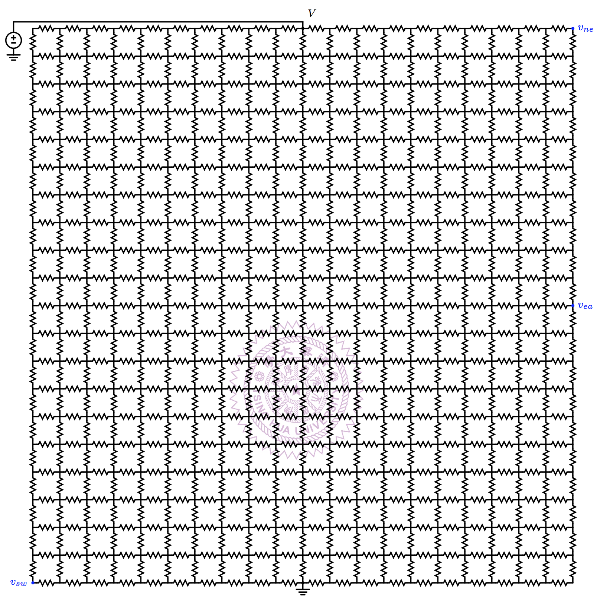
\includegraphics[width=0.5\textwidth]{src/network.png}
    \caption{Simple Resistor Network}
    \label{fig:network}
\end{figure}
For \textbf{Confugate Gradient Methods}, the error between iteration is defined as Equation \ref{eq:error}:
\begin{gather}
    Error = \sqrt{\frac{r^Tr}{n}}
    \label{eq:error}
\end{gather}
\newpage

\section{Implementation}
\begin{algorithm}[H]
    \caption{\textbf{Conjugate Gradient Methods}}
    \label{algo:cg}
    \begin{algorithmic}
        \State $p^{(0)} = r^{(0)} = b - Ax$
        \For{each iteration k $\in$ \{0, maxIter-1\}}
            \State $\alpha_k = \frac{(p^{k})^Tr^{(k)}}{(p^{k})^TAp^{k}}$
            \State $x^{(k+1)} = x^{(k)} + \alpha_kp^{(k)}$
            \State $r^{(k+1)} = r^{(k)} - \alpha_kAp^{(k)}$
            \State $\beta_k = \frac{(p^{(k)})^TAr^{(k+1)}}{(p^{(k)})^TAp^{(k)}}$
            \State $p^{(k+1)} = r^{(k+1)} - \beta_kp^{(k)}$
            \If{$\sqrt{\frac{(r^{(k+1)})^Tr^{(k+1)}}{n}} < tol$}
                \State break
            \EndIf
        \EndFor
    \end{algorithmic}
\end{algorithm}
\subsection{Complexity}
\label{sec:complexity}
For each iteration of Algorithm \ref{algo:cg}, the most time-consuming part is the multiplication of Matrix and Vector, which need a double for-loop.
As a result, this is a {\boldmath$O(n^2)$} problem.

\section{Discussion}
In this section, we will discuss the following issues:
\begin{enumerate}
    \item Why is Conjugate Gradient better than LU?
    \item Efficiency of Jacobi, Guass-Seidel, Symmetric Gauss-Seidel and Conjugate Gradient.
    \item Error of each iteration.
\end{enumerate}

\subsection{Conjugate Gradient vs LU Decomposition}
In the Discussion of homework03, we know that the complexity of LU Decomposition is $O(n^3)$, while each iteration of Conjugate Gradient is $O(n^2)$.
As a result, if the procedure of solving linear system needs small numbers of iteration, Conjugate Gradient can provide a much faster method to
solve Equation \ref{eq:system}. \newline
To compare the efficiency, I run several experiments for LU and CG. Table \ref{tab:LU} shows the result of LU, because of LU is too slow when N is
large, so the runtime after N $>$ 2601 is predicted by $O(n^3)$ and the three corner voltage value is provided by another classmate in this couse.
For Conjugate Gradient method, Table \ref{tab:cg} shows the detail result to achieve $10^{-7}$ error compared with LU Decomposition.

\begin{table}[htbp]
	\begin{tabular}{|c|c|c|c|c|c|c|c|c|}
		\hline
		\textbf{N} & 9 & 25 & 121 & 441 & 1681 & 2601 & 6561 & 10201 \\ \hline
		\textbf{Vne} & 0.75 & 0.7 & 0.648693 & 0.622178 & 0.603088 & 0.598084 & 0.588931 & no data \\ \hline
		\textbf{Vea} & 0.5 & 0.5 & 0.5 & 0.5 & 0.5 & 0.5 & 0.5 & no data \\ \hline
		\textbf{Vsw} & 0.25 & 0.3 & 0.351307 & 0.377822 & 0.396912 & 0.401916 & 0.411069 & no data \\ \hline
		\textbf{Runtime(s)} & 0.003 & 0.003 & 0.007 & 0.2 & 9.948 & 36.1 & 580(predict) & 2180(predict) \\ \hline
	\end{tabular}
	\caption{Experiment result of LU Decomposition}
	\label{tab:LU}
\end{table}
\begin{table}[H]
	\begin{tabular}{|c|c|c|c|c|c|c|}
		\hline
		\textbf{N} & 441 & 1681 & 2601 & 3721 & 6561 & 10201 \\ \hline
		\textbf{Iterations} & 75 & 148 & 184 & 221 & 293 & 365 \\ \hline
		\textbf{Vne} & 0.622178 & 0.603088 & 0.598084 & 0.594327 & 0.588931 & 0.585141 \\ \hline
		\textbf{Vea} & 0.5 & 0.5 & 0.5 & 0.5 & 0.5 & 0.5 \\ \hline
		\textbf{Vsw} & 0.377822 & 0.396912 & 0.401916 & 0.405673 & 0.411069 & 0.414859 \\ \hline
		\textbf{Runtime(s)} & 0.036 & 0.8 & 2.38048 & 5.96049 & 23.9501 & 73.0905 \\ \hline
		\textbf{iter\_avg} & 0.00048 & 0.0054054054 & 0.0129373913 & 0.026970543 & 0.0817409556 & 0.2002479452 \\ \hline
	\end{tabular}
	\caption{Experiment result of Conjugate Gradient}
	\label{tab:cg}
\end{table}

Figure \ref{fig:cg vs lu} shows \textbf{Runtime} in Table \ref{tab:LU} and \ref{tab:cg} vs N in log-scale. In this figure, we can see a significant 
efficiency gap between CG and LU. As a result, Conjugate Gradient is a better method for solving Simple Resistor Network.
\begin{figure}[H]
	\centering
	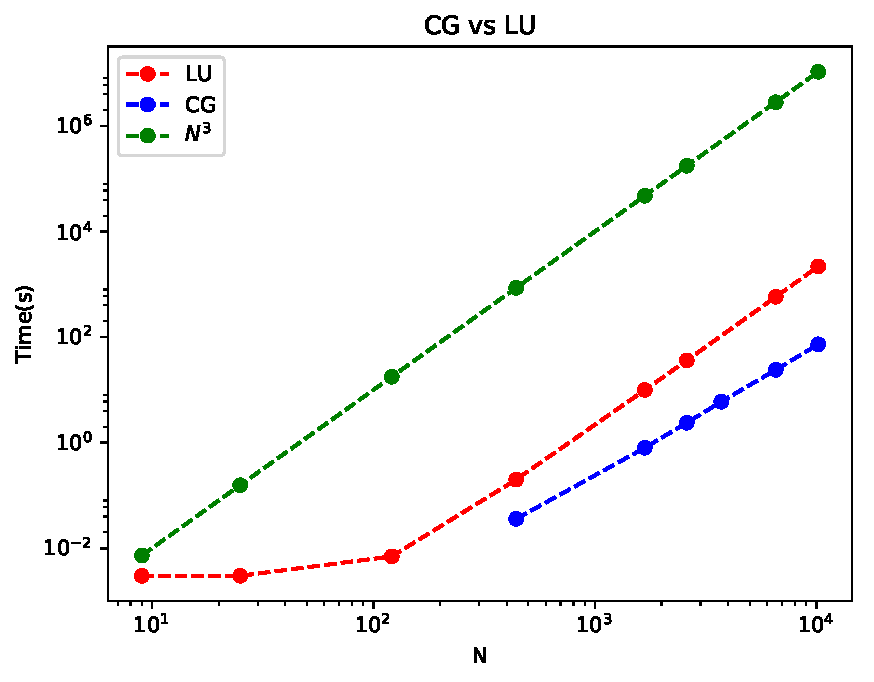
\includegraphics[width=0.7\textwidth]{src/cg_vs_lu.pdf}
	\caption{Comparison of CG and LU}
	\label{fig:cg vs lu}
\end{figure}

\subsection{Iterative Methods Comparison}
To do comparison between \textbf{Jacobi}, \textbf{Gauss-Seidel}, \textbf{Symmetric Gauss-Seidel} and \textbf{Conjugate Gradient}, the most
straightforward way is to comapre the number of iteration. Table \ref{tab:3 iter} show the result of iteration number.
\begin{table}[H]
	\begin{center}
		\begin{tabular}{|c|c|c|c|c|c|}
			\hline
			\textbf{N} & 9 & 25 & 121 & 441 & 1681 \\ \hline
			\textbf{Jacobi} & 62 & 310 & 2404 & 10892 & 47614 \\ \hline
			\textbf{Gauss-Seidel} & 32 & 155 & 1202 & 5441 & 23779 \\ \hline
			\textbf{SGS} & 23 & 90 & 628 & 2773 & 12007 \\ \hline
			\textbf{CG} & 4 & 10 & 37 & 75 & 148 \\ \hline
		\end{tabular}
	\end{center}
\caption{Iteration number of 3 algorithm}
\label{tab:3 iter}
\end{table}
Figure \ref{fig:iter comparison} shows the result with log-scale.
\begin{figure}[H]
	\centering
	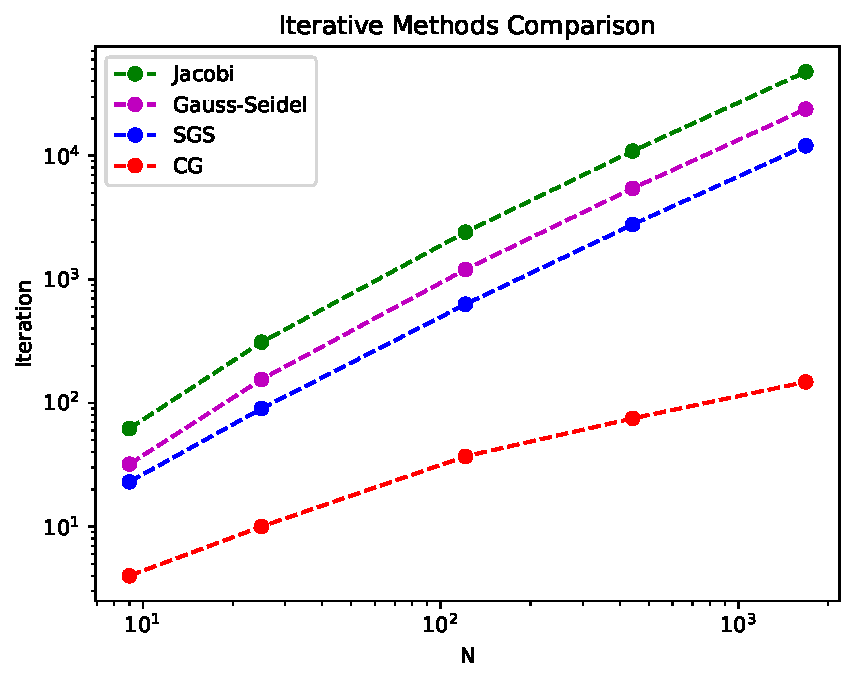
\includegraphics[width=0.7\textwidth]{src/iter.pdf}
	\caption{Comparison of 3 iterative methods}
	\label{fig:iter comparison}
\end{figure}
In Figure \ref{fig:iter comparison} we can see a dramatical drop of iteration number in Conjugate Gradient Method, which means CG can converge 
faster than the others. As a result, \textbf{Conjugate Gradient Method} is the best method for solving Simple Resistor Network.

\subsection{Iteration Error}
To see the trend of error, we can simply plot error of groundtruth(LU) and CG in each iteration. Figure \ref{fig:iter error} shows the result.
\begin{figure}[H]
	\centering
	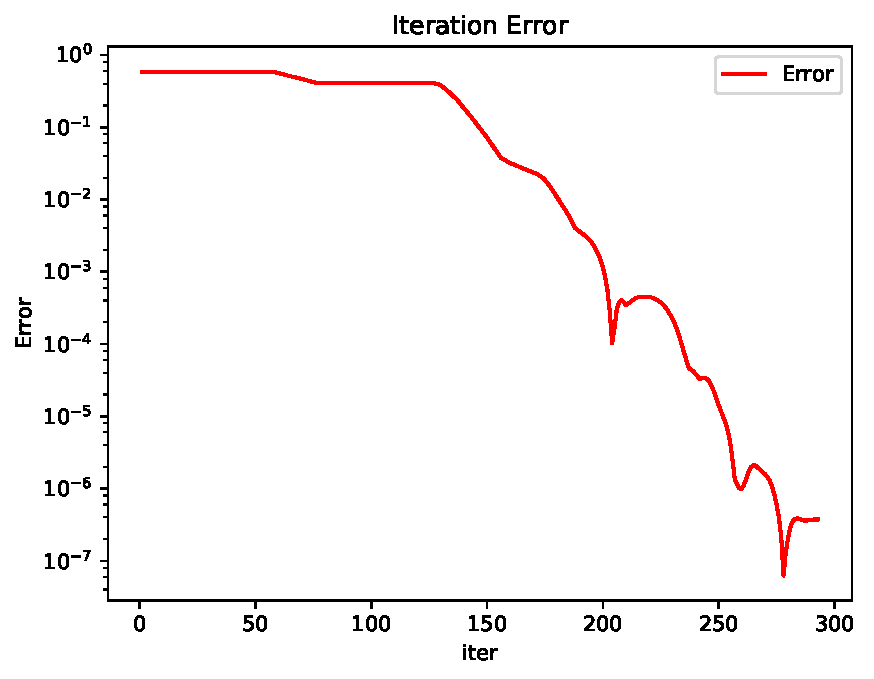
\includegraphics[width=0.7\textwidth]{src/iter_error.pdf}
	\caption{Iteration Error of Conjugate Gradient}
	\label{fig:iter error}
\end{figure}
In the begining, the error is almost a constant. After about 100 times of iteration, the error starts to drop with significant slope. This is 
because it was searching the right direction of convergence in the begining. After 100 iteration, it found the right direction. As a result
the converge speed increase a lot after that. About the time at 200 iteration, we can see the error starts to increase. This is because it 
adjusts the origin direction with an new one and make error increase in the begining. After several iteration, the error drop rate starts to
increase again and so on.




\end{document}













